\chapter{Future nEDM Measurement at TRIUMF}

Finding a non-zero neutron EDM is directly linked to the extra sources
of CP violation beyond the standard model. The TUCAN collaboration
proposes a world-leading experiment to measure the nEDM, improving the
precision by a factor of thirty compared to the present world’s best
experimental result. The current nEDM experiments suffer from low UCN
statistics. As a result, TUCAN has intended to build the strongest UCN
source in the world. To achieve this goal extensive studies of the
current vertical UCN source have been conducted~(See
Chapters~\ref{chap:UCNattriumf} and ~\ref{chap:UCNresult}).

To measure the neutron EDM, an ensemble of polarized UCN are put in
the presence of aligned electric and magnetic fields. The hamiltonian
of the interaction of the UCN with electric and magnetic fields are
described in Eqn.~\ref{eqn:hamiltonian}.  The larmor precession
frequency of UCN is then measured in two oriantations of parallel and
anti-parallel electric and magnetic fields. For the parallel $\bf{E}$
and $\bf{B}$ fields the Larmor precession frequency of UCN is written
as
\begin{equation}
\label{eqn:parallelEandB}
  h \nu_{\uparrow \uparrow} = 2 \mu_n \vert {\bf{B^{\uparrow \uparrow}}} \vert+ 2 d_n\vert \bf{ E^{\uparrow \uparrow}} \vert
\end{equation}
and for anti-parallel  $\bf{E}$ and $\bf{B}$ fields it is
\begin{equation}
\label{eqn:antiparallelEandB}
  h \nu_{\uparrow \downarrow} = 2 \mu_n \vert {\bf{B^{\uparrow \downarrow}}} \vert+ 2 d_n\vert \bf{ E^{\uparrow \downarrow}} \vert.
\end{equation}
Here $\uparrow \uparrow$ indicates the parallel Electric and Magnetic
fields and $\uparrow \downarrow$ represent the anti-parallel
orientation of those fields.
A nonzero nEDM is then extracted from any frequecy shift between these
two measurements:
\begin{equation}
  \label{eqn:dn}
  d_n = \frac{h \left( \nu_{\uparrow \uparrow} - \nu_{\uparrow \downarrow} \right) - 2 \mu_n \left( \vert {\bf{B^{\uparrow \uparrow}}} \vert -\vert {\bf{B^{\uparrow \downarrow}}} \vert \right)}{2 \left(\vert \bf{ E^{\uparrow \uparrow}} \vert - \vert \bf{ E^{\uparrow \downarrow}} \vert \right)}
\end{equation}
The main reason to employ this method is because it is impossible to
completely eliminate the $\bf{B}$ field to extract the neutron
EDM. These measurements are either performed in two adjacent volumes
with
$\vert E^{\uparrow \uparrow} \vert = - \vert E^{\uparrow \downarrow}
\vert$ and
$\vert B^{\uparrow \uparrow}\vert - \vert B^{\uparrow \downarrow} = 0
$ or measured in the same volume where the configuration of the fields
change in time. In the first case it is essential to make sure that
the magnetic field inside both volumes are the same and there is no
field gradient and in the second method it is essential to make sure
that the magnetic field is stable in time.

\section{Ramsey Method of Separated Oscillating
  Fields\label{sec:Ramsey}}

The Ramsey method of separated oscillating fields is the well-known
measurement technique to extract the neutron EDM. Ramsey obtained an
expression for the quantum mechanical transition probability of a
system between two states when the system subjected to such separated
oscillating
fields~\cite{ramsey1950}. Fig.~\ref{fig:ramsey}~\cite{Schmidt2016} left
shows a cycle of measurement. An ensemble of polarized UCN with the
inital spin $\ket{ \uparrow}$ are exposed to a DC magnetic field of
$B_0$.  A first RF pulse of $B_1 \cos (\omega_{rf}t)$ prependicular to
the $B_0$ field tips the spin of the neutrons to the transverse
plane. The neutrons precess freely with their Larmor precession
frequency $\omega_0$ for some time $T$ while accumulating a phase of
$\phi = \gamma_n BT$. Then again the second oscillating magnetic field
pulse of $B_1 \cos (\omega_{rf}t)$ is applied to the neutron
ensemble. The essential idea is to compare the phase $\phi$ with
$\omega_{rf}T$ and if they are identical then
$B= \omega_{rf} / \gamma_n$.

\begin{figure}[h]
  \centering
  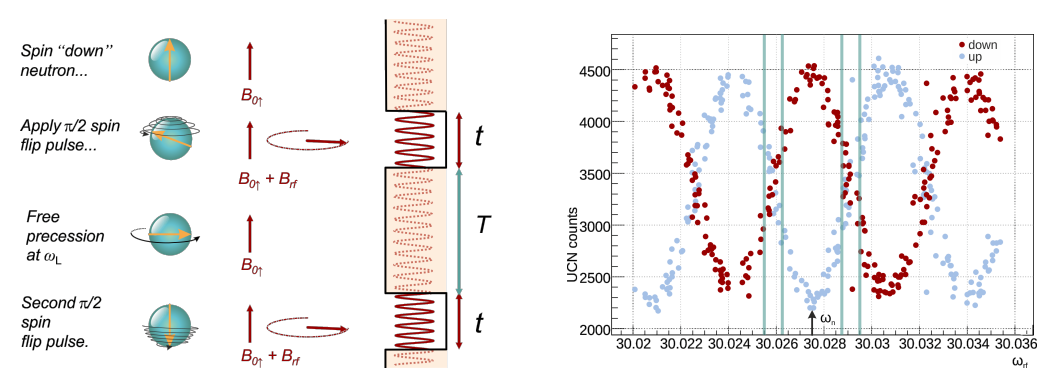
\includegraphics[width=1.0\textwidth]{ramsey.png}
  \caption{Ramsey method of separated oscillating fields. Left shows
    the scheme of a measurement procedure and right shows the data
    points. The blue points are the UCN counts with the spin up and
    the red points are the UCN with spin down (data from the PSI-nEDM
    collaboration). The width at half height~$\Delta \nu$ of the
    central fringe is approximately $1/2T$, the four vertical lines
    indicate the working points.}
  \label{fig:ramsey}
\end{figure}

The probability to find the UCN with spin up is
\begin{equation}
  \label{eqn:spinup}
  P(T, \omega_{rf}) = \bra{\uparrow} U(T, \omega_{rf}) \ket{\uparrow}
  = 1 - \frac{4 \omega_1^2}{\Omega^2} \sin ^2 \frac{\Omega t_{\pi/2}}{2} \left[ \frac{\Delta}{\Omega} \sin  \frac{\Omega t_{\pi/2}}{2} \sin \frac{T\Delta}{2} - \cos  \frac{\Omega t_{\pi/2}}{2} \cos\frac{T\Delta}{2} \right]^2,
\end{equation}
where $U(T, \omega_{rf})$ is the time evolutions operator,
$\omega_1 = - \gamma_n B_1$, $\Delta = \omega_{rf} - \omega_0$, and
$\Omega = \sqrt{\Delta^2 + \omega_1^2}$. When the spin-flipping pulses
are optimized we would have $\gamma_n B_1 t_{\pi/2} = \pi / 2$. In
this case the central fringe range ($\Delta \ll \omega_1$) and
Eqn.~\ref{eqn:spinup} simplifies to
\begin{equation}
  P(T, \omega_{rf}) = \frac{1}{2} \left( 1 - \cos(T\Delta) \right).
\end{equation}
In a real measurement with $N$ UCN inside a magnetic field region this
becomes
\begin{equation}
  \label{eqn:Nup}
N^{\uparrow} = \frac{N}{2} \left\lbrace 1 - \alpha(T) \cos \left[ (\omega_{rf} - \gamma_n B_0 ) \cdot \left(T+\frac{T+4t_{\pi/2}}{\pi}\right)\right]\right\rbrace,
\end{equation}
where $\alpha$ is the visibility of the central fringe with spin
either up or down
\begin{equation}
  \label{eqn:visibility}
  \alpha^{\uparrow /\downarrow} = \frac{N_{max}^{\uparrow /\downarrow} - N_{min}^{\uparrow /\downarrow}}{N_{max}^{\uparrow /\downarrow}+ N_{min}^{\uparrow /\downarrow}}.
\end{equation}
The term $4t_{\pi/2}/\pi$ is necessary to account for field
inhomogeneities of $B_1$ and $B_0$ which become relevant when the
pulse lenght $t_{\pi/2}$ is finite. The graph in Fig.~\ref{fig:ramsey}
shows the Ramsey interference pattern by scanning $\omega_{rf}$ while
everything else is kept the same. In actual nEDM measurements, only 4
points with the highest sensitivity are measured. These points are
refered to as the working points. For each configuration of the
electric and magnetic fields (parallel or anti-parallel)
Eqn.~\ref{eqn:Nup} is fitted to the data to extract the Larmor
frequency. Taking the differences of those Larmor frequencies then
give access to the neutron EDM
\begin{equation}
  \label{eqn:fitteddn}
  d_n = \frac{\hbar (\omega_0 ^{\uparrow \uparrow} - \omega_0 ^{\uparrow \downarrow})}{2(E^{\uparrow \uparrow} - E^{\uparrow \downarrow})} = \frac{\hbar \Delta \omega}{4E}.
\end{equation}
with the assumption that the magnetic field is constant~(see
Eqn.~\ref{eqn:dn}).


\section{Statistical and Systematic Errors}
\subsection{Statistical Sensitivity}
The statistical sensitivity of nEDM measurement per cycle is
\begin{equation}
  \label{eqn:dnsensitivity}
\sigma(d_n) = \frac{\hbar}{2 \alpha T E \sqrt{\bar{N}}}
\end{equation}
where visibility $\alpha$ is a factor related to the neutrons
polarization, $\bar{N}$ is the average total number of detected UCN,
$T$ is the free precession time and $E$ is the electric field. The
visibility depends on the longitudinal and transverse spin relaxation
times $T_1$ and $T_2$ respectively. The transverse spin relaxation
time $T_2$ arises from inhomogeneities in the magnetic field as well
as the $T_1$ relaxation time as
\begin{equation}
\frac{1}{T_2} = \frac{1}{T_2^{\prime}}+\frac{1}{T_1}
\end{equation}
where $T_2^{\prime}$ is the transverse relaxation time only
due to the field inhomogeneities.

\subsection{Systematic Errors}
The dominant systematic errors in the previous best experiment arose
due to magnetic field instability (uncorrelated with the electric
field E), and magnetic field inhomogeneity through the geometric phase
effect~(GPE)~\cite{pendlebury2004}~(see Appendix~\ref{app:GPE}).
%The GPE arises due to a combination of magnetic field
%inhomogeneity and motion of the particles in the electric field during
%the measurement time, when the neutrons and co-magnetometer atoms are
%confined in the trap. The spins of the species in the trap acquire
%phases relative to one another resulting in a false EDM
%signal.
The GPE could be understood by considering transverse fields
originating from the gradiant of the uniform $B_0$ field in the axial
direction~($\partial{B_{0z}}/\partial{z}$) and the motion of UCN in
the electric field~($\bf{B_v} =(\bf{E} \times \bf{v})/c^2 $),
respectively. Radial fields like these rotate as the particle moves in
the EDM cell.  These fields rotate with the same frequency as
particles move in the EDM cell, thereby inducing a Bloch-Siegert shift
on the resonant frequency. To analyze this effect, the field rotations
may be represented in terms of a perturbation on the precession
phase. The phase is shifted in 2nd order, resulting in a GPE. False
EDM effects arise from cross-terms between the radial component of the
applied $B_0$ field and $B_v$ in the 2nd order perturbation.

The false EDM could be corrected by the frequency ratio of the
neutrons to the co-magnetometer atoms~($^{199}$Hg) used to sense the
gradient. Graphing the measured neutron EDM as a function of this
ratio then allows to correct to zero gradient and hence discover the
true neutron EDM. This is also supplemented by gradient determination
using surrounding Cs magnetometers.


%This method can be calibrated for larger applied
%gradient fields. However, If the neutron resonant frequency is
%corrected by the co-magnetometer resonant frequency in the usual way,
%this results to false EDM for the neutrons induced by the
%co-magnetometer atoms. This type of false EDM could be reduced by
%using the buffer-gas effects to limit the mean free path $\lambda$ of
%the co-magnetometer atoms. If the mean free path of the atoms is
%limited, with interparticle collision times becoming small, a
%suppression factor may reduce the false EDM. If no buffer gas effect
%can be obtained for Xe, the simultaneous introduction of Hg and Xe
%atoms into the vessel can cancel out the GPE~(dual co-magnetometer).



\section{TRIUMF nEDM Components}
The future nEDM experiment at TRIUMF will use a room-temperature nEDM
apparatus, connected to a horizontal cryogenic UCN
source~Fig~\ref{fig:triumfEDM}.

A proton beam at 480~MeV and 40~$\mu$A impinges on a tungsten
spallation target liberating neutrons. Over the target a
room-temperature neutron moderator/reflector system composed of Pb,
graphite, and D$_2$O thermalizes the neutrons. Liquid
deuterium~(LD$_2$) at 20~K creates a large flux of cold neutrons~(CN)
in a bottle containing superfluid $^4$He below 1~K. In the superfluid,
the CN excite phonon and roton transitions, losing virtually all their
kinetic energy to become UCN. Once a sufficient density of UCN has
built up, the proton beam is turned off, and a cryogenic UCN valve
opens. The UCN are transported out of the source by specular
reflection on the surfaces of UCN guides. A superconducting
magnet~(SCM) accelerates polarized UCN through barrier foils to a
vacuum volume at room temperature. The UCN are then transported to the
nEDM experiment by additional guides.
%The cyclotron at TRIUMF produces a~$\sim$~500~MeV proton beam. Protons
%are guided to the spallation target using a variety of
%magnets. Spallation neutrons are moderated and converted to UCN in a
%superfluid He-II volume, which diffuse through UCN guides to the nEDM
%measurement cell.

In 2016 the vertical UCN source from RCNP in Japan was shipped to
TRIUMF for the resarch towards the developement of the new horizontal
UCN source.  The current UCN facility at TRIUMF is presented in
Chapter~\ref{chap:UCNattriumf}. The result of the first set of UCN
experiments with the vertical source is available in
Chapter~\ref{chap:UCNresult}.

\begin{figure}[h!]
  \centering
  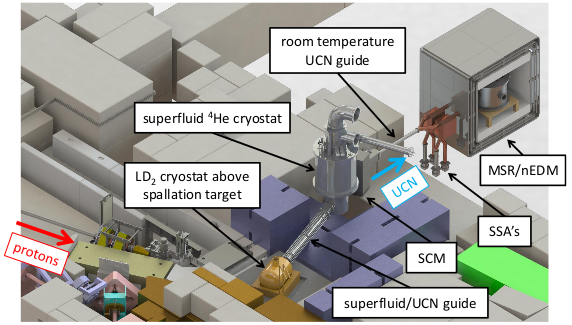
\includegraphics[width=1.0\textwidth]{edmtriumf.png}
  \caption{Conceptual design of the proposed UCN source and nEDM
    experiment. Protons strike a tungsten spallation target. Neutrons
    are moderated in the LD$_2$ cryostat and become UCN in a
    superfluid $^4$He bottle, which is cooled by another cryostat
    located farther downstream. UCN pass through guides and the
    superconducting magnet (SCM) to reach the nEDM experiment located
    within a magnetically shielded room (MSR). Simultaneous spin
    analyzers (SSA’s) detect the UCN at the end of each nEDM
    experimental cycle.  }
  \label{fig:triumfEDM}
\end{figure}

A brief description of the main
components of the future nEDM aparatus at TRIUMF is presented below.

\subsection{New UCN Source}
The future nEDM experiment at TRIUMF will use a new UCN source which
has quite some differences with the vertical UCN source described in
Chapter~\ref{chap:UCNattriumf}. A schematic overview of the proposed
UCN source upgrades and the nEDM experiment is presented in
Fig.~\ref{fig:triumfEDM}. The new UCN source uses an LD$_2$ cryostat
to produce cold neutrons during the experiment as opposed to the solid
D$_2$O in the vertical source. LD$_2$ increases the UCN production by
factors, and reduces the uncertainty in the UCN source performance. An
engineering diagram of the LD$_2$ cryostat connected to the superfluid
$^4$He cryostat is shown in Fig.~\ref{fig:newUCNsource}.

\begin{figure}[h!]
  \centering
  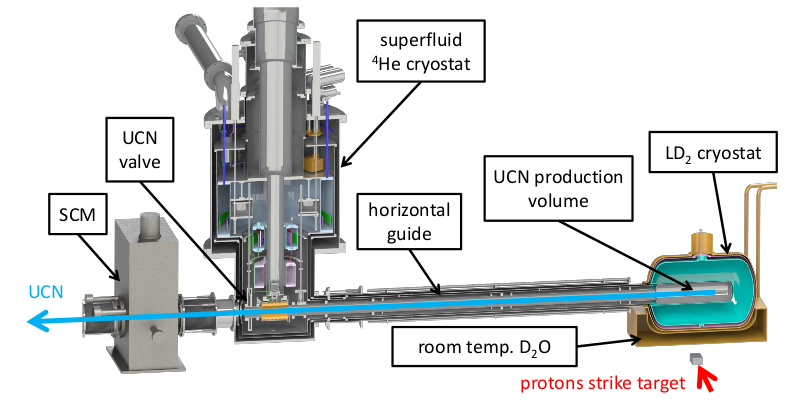
\includegraphics[width=1.0\textwidth]{newUCNsource.png}
  \caption{The proposed UCN source and LD$_2$ cryostat. Protons strike
    a tungsten spallation target liberating neutrons, which are
    moderated in surrounding volumes of graphite (not shown), D$_2$O,
    and LD$_2$. Neutrons are downscattered in the UCN production
    volume containing superfluid $^4$He. They are bottled within a
    horizontal guide up to a UCN valve. When the valve is opened UCN
    are transported to room temperature UCN guides.}
  \label{fig:newUCNsource}
\end{figure}





\subsection{UCN Handling and Transport}

Efficient transport of polarized UCN is one of the major requirements
for the measurement of the neutron EDM. This efficiency depends mainly
on three parameters.

The first one is the capacity of the guides walls to contain the
UCN. UCN have a large wavelength compared to the lattice constants in
solid matter~(50 to 130~nm compared to 0.3~nm). Therefore, during a
scattering process, a UCN interacts with hundreds of nuclei. The mean
nuclear potential experienced during the scattering, which is referred
to as the Fermi potential, depends on the material. In order to store
UCN, the Fermi potential must be as high as possible.

The second parameter is the roughness of the surface. Indeed,
transportation is more efficient if the roughness is low. Then, the
probability of having a specular reflection is increased. Empirically,
a roughnesses should be lower than the UCN wavelength.

The last parameter is related to the polarization. UCN can be
depolarized during a collision because of different processes.
%such as spin incoherent nuclear scattering, paramagnetic scattering or
%large magnetic field gradients.
When selecting materials for UCN components, the mean depolarization
rate per bounce should be as small as possible.
\begin{figure}[h!]
  \centering
  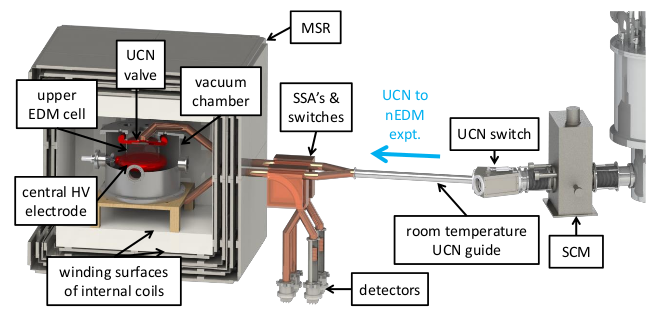
\includegraphics[width=1.0\textwidth]{UCNdelivery.png}
  \caption{UCN delivery and the nEDM experiment. UCN exit the source
    by passing through the SCM spin polarizer and UCN switch and
    detector system, where they then enter the proposed nEDM
    experiment. UCN are loaded into the measurement cells within a
    MSR/coil system. At the end of the measurement cycle, UCN are
    counted by simultaneous spin analyzers (SSA’s) including
    detectors. An ambient magnetic compensation system and thermally
    controlled room which will surround the nEDM apparatus (not
    shown). For scale, the innermost layer of the MSR is a 1.8~m
    side-length cube.}
  \label{fig:UCNdelivery}
\end{figure}



The main task of the UCN handling parts is to transport a large
phase-space fraction of the UCN most efficiently to achieve the
highest statistical sensitivity in the experiments as possible.

The parts that come in
contact with UCN on the way from the UCN source to the EDM experiment
and the UCN detectors constitute the neutron handling hardware: UCN
guides, valves, switches and simultaneous spin
analzer~(SSA) system. Fig.~\ref{fig:UCNdelivery} shows the neutron handling
parts for the nEDM experiment at TRIUMF.  UCN exiting the source are
polarized by the SCM, and then enter the nEDM experiment.

Suitable guides and valves have optimized geometries, wall materials
with large Fermi potentials, low upscattering and absorption cross
sections for neutrons, low roughness and depolarization. The plan is
to use Be for the UCN production volume, and NiMo coatings for most
other surfaces, on glass and Cu substrates where non-magnetic
polarization preserving guides are required.  

UCN spins will be measured by two separate simultaneous spin analyzer
(SSA) systems (one for each cell). Its configuration allows
simultaneous counting of both UCN spin states and maximizes the
visibility of the Ramsey fringes and counting efficiency.  The UCN
switches load UCN into the nEDM experiment, and divert UCN exiting the
experiment into the detectors.  A prototype detector, based on
scintillating lithium glass, and capable of handling the highest rates
of UCN expected with the TRIUMF source has been developed and tested
in the highest rate UCN beam available at
PSI~\cite{jamieson2017characterization}~(See
Chapter~\ref{chap:UCNattriumf}).
%This detector is based on the detector used
%in the PSI UCN experiments~\cite{Ban2009}.



%The cold neutron guides contain liquid helium (shown in purple in
%Fig.~\ref{fig:UCNhandling}) at a temperature of less than 1~K. A cold
%UCN gate valve partitions this volume. Upstream of it, the neutrons
%are stored/accumulated while the proton beam irradiates the
%target. Three aluminum foils constitute the end of the 1~K neutron
%guide section, sitting inside a 3.5~T superconducting magnet, the UCN
%polarizer. A transition region of guides bridges between temperatures
%from 100~K to room temperature, which is the temperature of all
%downstream neutron handling equipment.

%At TRIUMF, the room temperature UCN guide will be split between the
%EDM experiment and the second experiment port via a Y-switch. Towards
%the EDM cell(s), the UCNs pass another UCN switch (aka. rotary valve
%or EDM detector switch) which can either guide neutrons from the
%source to the EDM cell or from the EDM cell to the UCN detectors. Each
%EDM cell itself is closed by a plug (or door valve) to store the
%neutrons during the Ramsey cycle. The vertical section of the UCN
%guides towards the UCN detectors contains spin flippers and spin
%analyzers and the UCN detectors at the bottom.

%To systematically check all possible alignments of electric field,
%magnetic field and neutron spin in the EDM experiment, a spin flipper
%can be added to the UCN guide system after the Y-switch and before it
%is possibly split to serve the two EDM cells. In this way, both
%neutron spin states can be loaded into the experiment. The spin
%analyzer uses a magnetic potential of 60 neV/T to analyze the neutron
%spin direction, deter- mining whether it’s spin is aligned~(low field
%seekers), or anti-aligned~(high field seekers) with the analyzer
%magnetic field.





\subsection{Magnetic Components}
To chieve the desired sensitivity of ~$10^{-27}$~e$\cdot$cm an
extremely stable and homogeneuos $B_0$ magnetic field is required.
The magnetic stability upper limit for TUCAN's nEDM
measurement is 1~pT and the homogeneity of 1~nT/m.
%beyond which a comagnetometer must be
%used to correct the field to the $\sim$∼10~fT level.
Because of the challenges to achieve this level of magnetic stability,
a $^{199}$Hg co-magnetometer will be used to correct for the $B_0$
field fluctuations. To achieve these specifications, both active and
passive shielding will be utilized to nullify the uncontrolled and
time-varying external fields. The desired internal magnetic field will
be generated by using uniform and shim
coils. Fig.~\ref{fig:magneticscheme} shows the schematic drawing of
the magnetic components of the TUCAN nEDM experiment. Each magnetic
component is explained below.

\begin{figure}[h!]
  \centering
  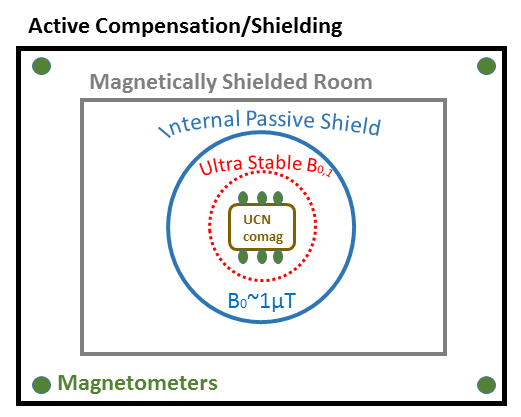
\includegraphics[width=0.7\textwidth]{magneticscheme.png}
  \caption{Schematic drawing for the TUCAN nEDM magnetics. From
    Outside in: The active compensation system followed by several
    layers of magnetically shielded room and passive shields nullify
    the environmental magnetic field. The magnetometers inside the
    active shielding monitor the changes in the magnetic field
    internal to that region. The internal coil system~($B_0$ and $B_1$
    coils) generate the magnetic fields for the Ramsey cycle. The UCN
    and the co-magnetometers are internal to the coils.  }
  \label{fig:magneticscheme}
\end{figure}



\subsubsection{Active Shielding}

The magnetic environment at the location of the planned nEDM
experiment at TRIUMF is dominated by a 400~$\mu$T static field due to
the main cyclotron at TRIUMF with 1 to 100~nT fluctuations due to the
other external magnetic sources such as the electrical equipment or
the displacement of large magnetic objects~(e.g., vehicle traffic).
The TUCAN's plan is to reduce the static field to less than 1~$\mu$T
using dedicated compensation coils and constant-current supplies with
a readily achievable steability of $10^{-3}$ and to reduce the
remaining static field and fluctuations by up to a factor of 100
through a separate set of compensation coils and current supplies
using fluxgate magnetometers for magnetic feedback. The fluxgate
sensors will be placed in the region between the compensation coils
and the passive shields as shown in Fig.~\ref{fig:magneticscheme}.  A
prototype active compensation system has been built at the University
of Winnipeg based on Refs.~\cite{beatrice,afach2014dynamic}. The
system employs a set of coils centered around a cylindrical passive
magnetic shield system using four 3-axis fluxgates for feedback~(See
Fig.~\ref{fig:prototype_active}). Overall, the active shielding
system should be able to reduce the net background magnetic field to
the level of tens of nT over the volume of the nEDM cell.


\subsubsection{Passive Shielding}
The passive shielding system nullifies the residual background fields
to the pT level. It will be a two-stage system: (1) a
magnetically shielded room~(MSR) with (2) a set of smaller shields
that fit inside the room and surround the nEDM apparatus.

A magnetically shielded room~(MSR) with quasi-static
shielding factor of $\sim$~100,000 is sufficient to reduce the magnetic
fluctuations to the $\sim$~pT level. A four-layer MSR with an inner
cubic space of side-length 1.8~m and outer side-length 2.8~m produces
this shielding factor, with mu-metal wall thicknesses 2~mm, 6~mm,
4~mm, 4~mm (inner to outer), equally spaced.


The innermost layer of the ineternal passive shields also serves as a
return yoke for the magnetic flux generated by the internal coils for
the shield-coupled coil desings. A degaussing~(idealization) system
will be used to stabilize the shields. A combined DC shielding factor
of the order of $10^6$ is expected. In principle, by utilizing both
active and passive shielding, the magnetic field from external sources
will be reduced to the level of tens of fT over the volume of the nEDM
cell.  There are two prototype four-layer passive shields at the
University of Winnipeg. The shields are now used to facilitate a
variety of magnetic field R\&D. These are made of high permeability
material. In addition, there are three small witness cylinders which
are made of the same material and annealed in the same oven as the
large passive shields. The design principles behind the small shield,
shielding factor measurements, and comparison to simulation are
described in Ref.~\cite{martin2015large}.  The witness cylinders are
used to evaluate the temperature dependence of the shield material
properties, which could be an important consideration for internal
field stability~(See Chapter~\ref{chap:muofT}).


\subsubsection{Internal Coils}
For internal coils, self-shielded $B_0$ coils and shim coils are
considered surrounding the nEDM cells since they provide immunity from
the field perterbations induced by changes in the magnetic
permeability of the passive shields arising from temperature
fluctuations~(See Chapter~\ref{chap:muofT}).  High-precision current
supplies ($\sim$~1~ppm) will be used to drive all internal coils,
regardless of design. AC coils will apply $\pi/2$ pulses for the UCN and
comagnetometer species, to initiate free spin precession.

%\textbf{also add field mapping and magnetometers???}


\subsection{ EDM Cells and High Voltage System}
The nEDM measurement volume, consists of two storage cells to enable
simultaneous measurements with both up and down orientations of the
electric field~(See Fig.~\ref{fig:HVcell}). The storage cells will be
housed inside a non-magnetic vacuum chamber providing insulating
vacuum for the high voltage applied to the central electrode which
separates the two cells.  The cells are separated by a cylindrical
wall of dielectric insulator.  The insulator must have a large
dielectric strength and low permittivity.  An electric field of
12~kV/cm will be created between the electrodes with minimal leakage
current~($<$~10 pA).  The optical readout of the comagnetometer
requires UV-transparent windows in the insulating side wall. The use
of two cells with a central electrode allows first-order compensation
of magnetic field drifts and a measurement of the magnetic field
gradient.

\begin{figure}[h!]
  \centering
  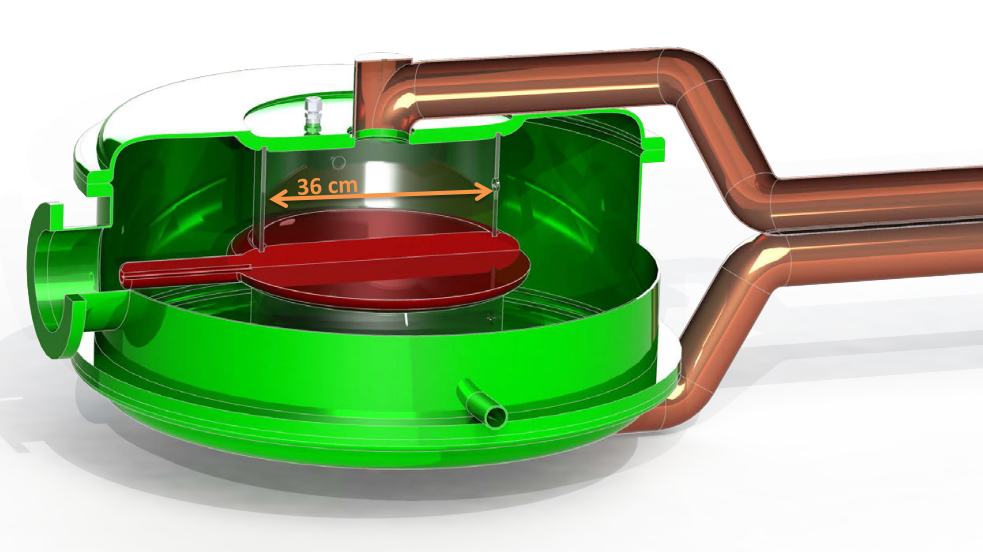
\includegraphics[width=0.7\textwidth]{HVcell.png}
  \caption{3D drawing of the double EDM cell with vacuum chamber and
    UCN guides}
  \label{fig:HVcell}
\end{figure}



\subsection{Comagnetometry}
A false nEDM signal may arise due to a combination of a magnetic field
gradient $\partial {B_z}/\partial z$ and motion in the electric field when
species (neutrons and $^{199}$ Hg atoms) are confined in the
measurement cells. Comagnetometry offers the only way to correct for
false EDMs caused by leakage currents.  Each $^{199}$Hg atom is
polarized using optical pumping techniques. Polarized atoms are
introduced into the nEDM cell at the same time as UCN, and the
spin-precession frequencies of them are measured simultaneously. The
atoms are expected to have smaller EDMs than the neutrons, and so
their precession frequencies may be used to normalize magnetic field
drifts.  The design of the $^{199}$Hg comagnetometer will be similar
to that employed in the previous ILL
experiment~\cite{Baker2006,Griffith2009}.

%%%%%%%%%%%%%%%%%%%%%%%%%%%%%%%%%%%%%%%%%%%%%%%%%
%% repeating myself
%%%%%%%%%%%%%%%%%%%%%%%%%%%%%%%%%%%%%%%%%%%%%%%%%
%\subsection{UCN Handling and Transport}
%Fig.~\ref{fig:UCNdelivery} shows the UCN transport to the EDM cell.
%UCN will be transported out of the source by specular reflection via
%guides with special coatings compatible with UCN transport and
%polarization. Special coatings such as NiMo, NiP and DLC are top
%candidates because of their high Fermi potential , small absorption
%and inelastic upscattering, and good specularity.  A superconducting
%magnet (SCM) accelerates polarized UCN through barrier foils to a
%vacuum volume at room temperature. The UCN are then transported to the
%nEDM experiment by additional guides.



%\begin{figure}[h!]
%  \centering
%  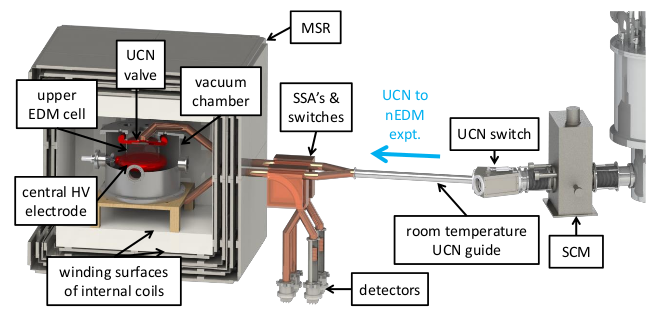
\includegraphics[width=1.0\textwidth]{UCNdelivery.png}
%  \caption{UCN delivery and the nEDM experiment. UCN exit the source
%    by passing through the SCM spin polarizer and UCN switch and
%    detector system, where they then enter the proposed Phase 2 nEDM
%    experiment. UCN are loaded into the measurement cells within a
%    MSR/coil system. At the end of the measurement cycle, UCN are
%    counted by simultaneous spin analyzers (SSA’s) including
%    detectors. An ambient magnetic compensation system and thermally
%    controlled room which will surround the nEDM apparatus~(not
%    shown). For scale, the innermost layer of the MSR is a 1.8~m
%    side-length cube.}
%  \label{fig:UCNdelivery}
%\end{figure}



%\subsection{DAQ?}
%\begin{description}
%\item{An introduction about the long term nEDM effort at TRIUMF, what
% the plan is, when it will start (roughly). I guess I can probably
% get this information from some proposals. I am not sure how much
% detail should go here.}
  
%\item{How the EDM experiment is actually done, talk about different
%  components of the system. Here is where I talk about the Ramsey
%  cycle ...}
  
%\item{nEDM measurement systematic effects: This is where I talk about
%  the GPE and ... . Basically here is to kind of motivate that we need
%  to have stable magnetic fields and we need lots of neutrons.}
  
%\item{Introduction to the magnetic stability requirements at
%  TRIUMF. What I mean is that there is 400 $\mu$T background field at
%  TRIUMF. Hopefully we have a field map of the area soon(?).}
  
%\item{From ouside in: Magnetically shielded room, what is the status
%  of that, are we going to have it? when? How good is it going to be
%  compared to the other ones worldwide? Why is it designed that way?
%  What is the design? Drawings of it. General question: Some of these
%  are about things that will happen in the future and I have not
%  worked on them. Should they even go to my thesis? I feel I have to
%  say a little about this since my thesis is nEDM related and it is
%  part of it.}
  
%\item{Passive shieldings: Again same questions as above, motivate for
%  the next chapter}

  
%\item{Say what will be discussed in the two coming chapters}
  
%\item{what else?}
%\end{description}